%%
%% This is file `sample-sigconf.tex',
%% generated with the docstrip utility.
%%
%% The original source files were:
%%
%% samples.dtx  (with options: `sigconf')
%% 
%% IMPORTANT NOTICE:
%% 
%% For the copyright see the source file.
%% 
%% Any modified versions of this file must be renamed
%% with new filenames distinct from sample-sigconf.tex.
%% 
%% For distribution of the original source see the terms
%% for copying and modification in the file samples.dtx.
%% 
%% This generated file may be distributed as long as the
%% original source files, as listed above, are part of the
%% same distribution. (The sources need not necessarily be
%% in the same archive or directory.)
%%
%% Commands for TeXCount
%TC:macro \cite [option:text,text]
%TC:macro \citep [option:text,text]
%TC:macro \citet [option:text,text]
%TC:envir table 0 1
%TC:envir table* 0 1
%TC:envir tabular [ignore] word
%TC:envir displaymath 0 word
%TC:envir math 0 word
%TC:envir comment 0 0
%%
%%
%% The first command in your LaTeX source must be the \documentclass command.
\documentclass[sigconf,review,anonymous]{acmart}
%\acmConference[ESEC/FSE 2022]{The 30th ACM Joint European Software Engineering Conference and Symposium on the Foundations of Software Engineering}{14 - 18 November, 2022}{Singapore}
%% NOTE that a single column version may be required for 
%% submission and peer review. This can be done by changing
%% the \doucmentclass[...]{acmart} in this template to 
%% \documentclass[manuscript,screen]{acmart}
%% 
%% To ensure 100% compatibility, please check the white list of
%% approved LaTeX packages to be used with the Master Article Template at
%% https://www.acm.org/publications/taps/whitelist-of-latex-packages 
%% before creating your document. The white list page provides 
%% information on how to submit additional LaTeX packages for 
%% review and adoption.
%% Fonts used in the template cannot be substituted; margin 
%% adjustments are not allowed.
%%
%%
%% \BibTeX command to typeset BibTeX logo in the docs
\AtBeginDocument{%
  \providecommand\BibTeX{{%
    \normalfont B\kern-0.5em{\scshape i\kern-0.25em b}\kern-0.8em\TeX}}}

%% Rights management information.  This information is sent to you
%% when you complete the rights form.  These commands have SAMPLE
%% values in them; it is your responsibility as an author to replace
%% the commands and values with those provided to you when you
%% complete the rights form.
%\setcopyright{acmcopyright}
%\copyrightyear{2018}
%\acmYear{2018}
%\acmDOI{XXXXXXX.XXXXXXX}

%% These commands are for a PROCEEDINGS abstract or paper.
%\acmConference[Conference acronym 'XX]{Make sure to enter the correct
%  conference title from your rights confirmation emai}{June 03--05,
%  2018}{Woodstock, NY}
%
%  Uncomment \acmBooktitle if th title of the proceedings is different
%  from ``Proceedings of ...''!
%
%\acmBooktitle{Woodstock '18: ACM Symposium on Neural Gaze Detection,
%  June 03--05, 2018, Woodstock, NY} 
\acmPrice{15.00}
\acmISBN{978-1-4503-XXXX-X/18/06}


%%
%% Submission ID.
%% Use this when submitting an article to a sponsored event. You'll
%% receive a unique submission ID from the organizers
%% of the event, and this ID should be used as the parameter to this command.
%%\acmSubmissionID{123-A56-BU3}

%%
%% For managing citations, it is recommended to use bibliography
%% files in BibTeX format.
%%
%% You can then either use BibTeX with the ACM-Reference-Format style,
%% or BibLaTeX with the acmnumeric or acmauthoryear sytles, that include
%% support for advanced citation of software artefact from the
%% biblatex-software package, also separately available on CTAN.
%%
%% Look at the sample-*-biblatex.tex files for templates showcasing
%% the biblatex styles.
%%

%%
%% The majority of ACM publications use numbered citations and
%% references.  The command \citestyle{authoryear} switches to the
%% "author year" style.
%%
%% If you are preparing content for an event
%% sponsored by ACM SIGGRAPH, you must use the "author year" style of
%% citations and references.
%% Uncommenting
%% the next command will enable that style.
%%\citestyle{acmauthoryear}


\usepackage{minted}
\usepackage{fontawesome}
\usepackage{tikz}
\usepackage{tikz-network}
\usepackage{xspace}
\usemintedstyle{emacs}

\newcommand{\code}[1]{%
  \mintinline[fontsize=\footnotesize{},mathescape, escapeinside=||]{c}{#1}%
}

\definecolor{taintcolor}{rgb}{0.87, 0.36, 0.51}

\newcommand{\tbl}[1]{Table~\ref{#1}}
\newcommand{\sect}[1]{Section~\ref{#1}}
\newcommand{\fig}[1]{Figure~\ref{#1}}
\newcommand{\lst}[1]{Listing~\ref{#1}}
\newcommand{\algo}[1]{Algorithm~\ref{#1}}
\newcommand{\apdx}[1]{Appendix~\ref{#1}}

\newcommand{\realbug}{\textcolor{red}{\faBug}}
\newcommand{\complexcode}{\faChainBroken}
\newcommand{\entrypoint}{\faForward}
\newcommand{\rootcause}{\textcolor{orange}{\faWarning}}
\newcommand{\useradded}{\faUserPlus}
\newcommand{\usermods}{\faUser}

\newcommand{\ptr}{\ensuremath{ptr}}
\newcommand{\arr}{\ensuremath{arr}}
\newcommand{\ntarr}{\ensuremath{ntarr}}
\newcommand{\ptrT}[1]{\code{ptr<#1>}}
\newcommand{\arrT}[1]{\code{array_ptr<#1>}}
\newcommand{\ntarrT}[1]{\code{nt_array_ptr<#1>}}
\newcommand{\ucregion}{\ensuremath{uc-region}\xspace}
\newcommand{\cregion}{\ensuremath{c-region}\xspace}
\newcommand{\taintt}{\code{t_*}}

\newcommand{\aravind}[1]{\textcolor{green}{Aravind: #1}}


\newcommand{\systemname}{\textsc{CheckCBox}\xspace}

%%
%% end of the preamble, start of the body of the document source.
\begin{document}

%%
%% The "title" command has an optional parameter,
%% allowing the author to define a "short title" to be used in page headers.
% This is the CFP: https://conf.researchr.org/track/ase-2022/ase-2022-nier-track
\title{Incremental Spatial Memory Safety with~\systemname}

%\setcopyright{none}

%%
%% The "author" command and its associated commands are used to define
%% the authors and their affiliations.
%% Of note is the shared affiliation of the first two authors, and the
%% "authornote" and "authornotemark" commands
%% used to denote shared contribution to the research.

%%
%% By default, the full list of authors will be used in the page
%% headers. Often, this list is too long, and will overlap
%% other information printed in the page headers. This command allows
%% the author to define a more concise list
%% of authors' names for this purpose.

%%
%% The abstract is a short summary of the work to be presented in the
%% article.
\begin{abstract}
  A clear and well-documented \LaTeX\ document is presented as an
  article formatted for publication by ACM in a conference proceedings
  or journal publication. Based on the ``acmart'' document class, this
  article presents and explains many of the common variations, as well
  as many of the formatting elements an author may use in the
  preparation of the documentation of their work.
\end{abstract}

%%
%% The code below is generated by the tool at http://dl.acm.org/ccs.cfm.
%% Please copy and paste the code instead of the example below.
%%


%\ccsdesc[500]{Computer systems organization~Embedded systems}
%\ccsdesc[300]{Computer systems organization~Redundancy}
%\ccsdesc{Computer systems organization~Robotics}
%\ccsdesc[100]{Networks~Network reliability}

%%
%% Keywords. The author(s) should pick words that accurately describe
%% the work being presented. Separate the keywords with commas.
%\keywords{datasets, neural networks, gaze detection, text tagging}

%% A "teaser" image appears between the author and affiliation
%% information and the body of the document, and typically spans the
%% page.

%%
%% This command processes the author and affiliation and title
%% information and builds the first part of the formatted document.
\maketitle

\section{Introduction}\label{sec:intros}

Vulnerabilities due to memory corruption, especially spatial memory corruption, 
are still a major issue for C programs~\cite{cvetrend, microsoftmemsafe, Zeng:2013:SRF:2534766.2534798} 
despite many efforts that tried to prevent them~\cite{song2019sanitizing}.
Several industrial and research efforts, including CCured~\cite{Necula2005},
Softbound~\cite{softbound}, and ASAN~\cite{Serebryany2012},
have investigated ways to better compile C programs with automatic safety enforcement.
These approaches impose performance overheads deemed too high for deployment use, especially for resource-constrained embedded systems.
%
Previous works~\cite{meng2021bran, du2019leopard} show that vulnerabilities are not uniformly distributed in real programs.
Some components/functions are likelier to have a certain class of vulnerabilities.
\eg{} spatial safety issues in string processing functions.
have.

Program partitioning is a well-known technique that enables separating potentially vulnerable functions (untrusted region) from the rest of the program (trusted region).
%
Several automated program partitioning techniques~\cite{tan2017principles, brumley2004privtrans, bittau2008wedge, lind2017glamdring, liu2017ptrsplit} exist, but they have a considerable performance overhead. 

One of the main reasons for this is combining partitioning with~\acf{SFI}~\cite{wahbe1993efficient}.
Specifically, in addition to partitioning, existing techniques also provide~\ac{SFI} such that code in the untrusted region cannot affect code in the trusted region,~\eg{} by executing untrusted partition in a separate process~\cite{liu2017ptrsplit} or executing in a Trusted Execution environment~\cite{lind2017glamdring}.
However, this extreme partitioning is not always necessary and feasible in certain resource constrained environments.
For instance, we want to isolate a string processing function only from spatial violations,~\ie any spatial violations (\eg buffer overread) in that function should not affect the program.
%
But existing partitioning techniques are specialized for a specific~\ac{SFI} technique (\sect{subsec:background:programpart}).
%For instance,~\ptrsplit{}~\cite{liu2017ptrsplit} technique assumes that partitions are hosted as separate processes and data is exchanged through marshaling.
%Any other isolation mechanism or data exchange (\eg shared memory) cannot be supported as the partitioning technique is specialized for marshaling by using~\ac{PDG} and tracking bounds information.

In other words, existing techniques combine policy (\ie{}~\emph{what} to partition) with mechanism (\ie{}~\emph{how} to partition).
We argue that existing program partitioning mechanisms are restrictive and inflexible for different use cases (\eg isolation from spatial safety vulnerabilities). We need a technique that enables developers to flexibility partition programs and enforce isolation -- balancing safety guarantees and performance overhead.

In this paper, we present~\systemname{}, a Type Directed Flexible Program Partitioning system.
The main design principle of the system is to separate partitioning (\ie policy) from enforcing the separation between partitions (\ie mechanism).
Once a program is partitioned, users can choose enforcement mechanisms based on the desired guarantees and tolerable performance overhead. For instance, for the same program, the user may use complete~\ac{SFI} for desktop systems v/s isolation against only spatial safety issues on embedded systems.

We propose a type directed partitioning through untrusted types.
Specifically, we introduce~\textbf{tainted} (\taintt) qualifiers that can be used to annotate pointer types or functions. 
The tainted types form the untrusted partition or~\umode~\emph{region} (can only access tainted types), and the non-tainted types will be the trusted partition or~\cmode~\emph{region} (has complete access).
Through static type checking, our type system ensures that tainted types cannot directly affect untainted types.
After successful type checking,~\systemname{} creates two sets of source files:~\ucregion{} and~\cregion{}, containing tainted and untainted entities, respectively.

%These sets of source files will be compiled using~\systemname{} compiler, which enforces the desired isolation through instrumentation.
%Developers can choose a specific isolation mechanism.
These sets of source files will be compiled using~\systemname{} compiler, which enforces a selected isolation mechanism.
We introduce the concept of~\emph{\acf{SeFI}} and explore four different isolation mechanisms with varying guarantees and performance overhead (CITE SECTION).
For instance,~\isoheap{} provides safety against spatial and temporal violations of tainted pointers with almost~\emph{no} performance overhead.
Whereas~\sandbox{} isolation provides complete~\ac{SFI} with~\avgsandboxoverhead{} runtime overhead.

%Our dynamic instrumentation ensures that tainted pointer accesses are valid according to the desired isolation mechanism.
\noindent\textbf{Formal Guarantee.} We formally prove the~\emph{clean separation theorem} that guarantees that tainted types are isolated from the rest of the programs in a well-typed program.
The specific isolation guarantee depends on the target~\ac{SFI} mechanism.

In addition to the flexibility, the type based partitioning has the following advantages:

\noindent\textbf{Interactive Partitioning.} Our type system enables interactive partitioning, wherein developers start by annotating a risky pointer (\ie{} user data), and our type system will identify all the other additional pointers (depending on the tainted pointer) that need tainted or sanitized (\eg by explicitly copying to untainted buffer).

\noindent\textbf{Integrating with Other Mechanisms.} Using types enables us to integrate easily with existing type based safety mechanisms. We demonstrate this by combining~\systemname{} with~\checkedc, which we call~\ccflex.
\checkedc~\cite{Elliott2018} provides backward-compatible spatial safety by using checked pointer types. 
But, as we explain in~\sect{subsec:nosafetyagsintuncheckedcode}, the unchecked (or wild) pointers in a~\checkedc program are prone to cross-language attacks~\cite{mergendahl2022cross} and can violate the whole program's spatial safety.
However, using~\systemname{}, one can mark all unchecked (or wild) pointers as tainted, thus partitioning away unchecked types.
These unchecked components can be executed in an isolated sandbox, thereby preventing cross-language attacks and upholding~\checkedc guarantees.

Our evaluation shows that ---complete this. \aravind{Complete this.}

In summary following are our contributions:

\myparagraph{\systemname Type System and Formalism}
We designed and implemented a flexible program partition technique using tainted types.
Our type system guarantees that the tainted pointers cannot affect untainted pointers and partition the given code into~\ucregion (containing only tainted entities) and~\cregion (CITE SECTION).
We provide formal proof of the~\emph{clean separation theorem} that guarantees that code in ~\cregion will be separated from~\ucregion according to the target isolation mechanism (CITE SECTION).
We also integerated~\systemname{} with~\checkedc that provides additional~\emph{non-crashing} and \emph{non-exposure} guarantees (CITE SECTION).

\myparagraph{Flexible Isolation Mechanisms and Implementation}
We introduce the concept of~\emph{\acf{SeFI}} and designed four isolation mechanisms with varying guarantees and performance overhead, providing flexibility in choosing a desired isolation mechanism (CITE SECTION).
We implemented our type system (CITE SECTION) and flexible partitioning (CITE SECTION) by modifying~\clang{} compiler.

\myparagraph{Evaluation}
Our evaluation on ...

We made our implementation and datasets open-source to foster future research. 

\iffalse
 
% 
%\liyi{Should we say this? Is the paper about overhead reducing? }
Recently,~\citet{Elliott2018} and~\citet{li22checkedc} introduced and formalized \checkedc, an
open-source extension to C,
to ensure a program’s spatial safety by introducing new pointer types,~\ie checked ($\cmode$) pointer types.
%
The checked pointers are represented as system-level memory words without ``fattening'' metadata~\cite{duck2016heap}, 
and ensuring backward compatibility,~\ie developers can use checked and regular (unchecked $\umode$) pointers within the same program.
%users are able to split code into checked and unchecked regions and incrementally convert
%C code in the unchecked region to Checked C code in the checked one.
However, as we explain in~\sect{subsec:nosafetyagsintuncheckedcode}, the
unconverted or unchecked ($\umode$) code can violate guarantees provided in $\cmode$
regions.
%
We need to ensure that~\emph{code executed as part of 
unchecked ($\umode$) regions does not lead to the safety violations in checked ($\cmode$) regions  with the use of program partitioning mechanism \cite{rul2009towards}}.

% One possible solution is Checked C
% \begin{itemize}
% \item Think of it as migratory/gradual typing, but for C.
% \item Distinct pointer types, but which are backward binary- and source-compatible.
% \item Checked regions, containing only checked pointers and restricted
%   idioms, aim to ensure spatial safety
% \item Implemented as an extension to Clang/LLVM. Good performance
%   (compared to ASAN etc.)
% \end{itemize}
\iffalse
\noindent
\textbf{No safety against unchecked code.} The \checkedc spatial safety guarantee applies to completely converted programs, i.e., programs that uses only checked types.
Although, the backward compatibility of Checked C helps a partially annotated program to enjoy spatial memory safety on those regions using only Checked pointers (i.e., checked or safe regions).
But, the unconverted code regions (or unsafe regions) can affect pointers in safe regions and violate certain assumptions leading to vulnerabilities, as demonstrated by cross-language attacks~\cite{mergendahlcross}.
Although the blameless proof exists~\cite{ruef2019achieving} for~\checkedc, it does not state that spatial safety violations cannot happen in Checked regions but rather states that Checked regions~\emph{cannot be blamed for any spatial safety violations}.
Consider the following example:
\begin{minted}[xleftmargin=25pt, mathescape, linenos, escapeinside=||, fontsize=\footnotesize{}]{c}
// Checked code
int func(array_ptr<char> p : count(5)) {
|\textcolor{red}{\faChainBroken}|..p[4]..
}
// unchecked code
...
str = "he";
...
|\textcolor{red}{\faBug}|assume_bounds_cast<char>(str, 5); 
...
char ptr[16];
...
len <- derived from user input
...
|\textcolor{red}{\faBug}| memcpy(ptr, buff, len); // buffer overflow
\end{minted}
Here, the checked function~\inlinecode{func} expected a pointer to a buffer of five elements, but unchecked code violated it and invoked the function with a buffer of 2 elements.
This results in a spatial safety violation (\textcolor{red}{\faChainBroken}) in the Checked region, but of course, the blame or the root cause is in the unchecked region (\textcolor{red}{\faBug}).
Furthermore, since checked and unchecked regions execute in the same address space, spatial memory corruptions in unchecked regions (Line 15) can take down the complete program despite having checked regions.
We need~\emph{an isolation mechanism to ensure that code executed as part of unchecked regions does not violate the safety guarantees in checked regions}.
\fi
% 

Existing such mechanisms are not suitable as they are based on process isolation and have high overhead, and are \emph{data-centric} (\sect{subsec:background:programpart}).
%Furthermore, these techniques are hard to engineer to co-exist with~\checkedc.
%\liyi{why? Can we not say this? It seems that the whole reason people should care our work is we did it in \checkedc, but \checkedc itself is the selling product here.... }
But in our case, we want a low-overhead code-centric partitioning, where the $\umode$ region code (or functions) should be isolated (or partitioned) from $\cmode$ one. We also want the technique to co-exist and be compatible with Checked C guarantees such that the partition containing $\cmode$ region code can maintain spatial safety.

Here, we propose a type-directed code-centric program partitioning approach.
Specifically, our system,~\systemname, extends \checkedc's checked and unchecked pointer types---representing safe and unsafe program pieces---with \textbf{tainted} (\taintt) types running on an isolated sandbox mechanism,
forbids the communication between checked and unchecked type entities, and enforces the communication between checked and unchecked types
through the uses of tainted types with additional validity checks. 
%which can be used to mark functions and pointers that need to be isolated from the original program, while checked types follow the standard \checkedc typing rules.
%However, our type-system disallows any unsafe interactions between taint and untainted types.
% 
% Specifically, in our system,~\systemname, extending CheckedC,
% functions and pointers that need to be isolated from the original program can be
% marked with ~\textbf{tainted} (\taintt) types.
% 

The developer starts by marking desired (\ie unchecked, $\umode$) functions and pointers used in functions as tainted. 
Then, \systemname partitions the given program into two partitions (\umode and~\cmode regions) of different privileges:

\begin{itemize}
\item~\umode \emph{region} (low privilege tainted region, extended from the unchecked region in \checkedc): this partition contains tainted types (\ie functions and pointers) and can only access tainted and unchecked pointers.
\item~\cmode \emph{region} or~\emph{safe region} (high privilege untainted or checked region): This partition contains the remaining (untainted) code and data and has complete access to~\cmode region.
The functions in~\cregion can invoke any function in~\ucregion and access all its data but not the other way around, except for call-back functions, which we will discuss later.
\end{itemize}

The $\cmode$ region code is executed as a regular program, while the~\ucregion partition will be executed in an existing sandboxed environment (\eg WASM sandbox), with additional instrumentations to facilitate the communication between code in~$\cmode$ and~$\umode$ regions.

The combination of tainted types and privileged partitions
enforces isolation and provides memory safety without transforming all unchecked C code to \checkedc code,
because unchecked types can stay in \ucregion, and \cregion code can access tainted type entities that are allocated 
in \ucregion.
% 
Although memory isolation prevents direct violations,~\ucregion code can still affect~\cregion through tainted pointers by confused deputy attacks~\cite{rajani2016access, machiry2017boomerang},~\eg by using a valid~\cregion address in a tainted pointer.
Our compiler avoids these attacks by ensuring using dynamic checks that tainted pointers validly point to~\ucregion address space.
Such checks are statically generated by our compiler.

In summary, we make the following three main contributions.

\myparagraph{\systemname Type System, Formalism and Compiler}
We present a type system that integrates tainted types with~\checkedc and provides additional guarentees---the~\emph{non-crashing} and \emph{non-exposure} guarantees,~\ie a well-typed~\systemname program can never crash due to spatial safety violations,
as well as \ucregion code cannot directly observe a checked pointer address.
%no \cregion pointer addresses will be leaked in
%\ucregion code
We extend the \checkedc compiler to support the type system and
formalize it by extending~\checkedc formalism~\cite{li22checkedc} with the non-crashing and non-exposure guarantees.
We formally prove theorems related to the two guarantees and use model-based randomized testing \cite{Pierce:SF4} to certify the simulation relation between the~\systemname semantics and its compiler formalism.
To the best of our knowledge,~\systemname is the first C(-like) language and compiler formalism with the program partitioning mechanism.

\myparagraph{Type-Directed Program Partitioning}
We present a type-directed program partition technique to separate $\cmode$ and $\umode$ code regions and ensure the above guarantees.
%Our type system restricts checked pointers usage only in~\cregion and ensures that~\ucregion can only access tainted pointers.
Our modular design enables us to use existing sandbox techniques to enforce memory and execution isolation, with the implementation of tainted pointers in the \systemname compiler.

\myparagraph{Supporting callbacks to~\cregion with no Checked Pointer Exposure}
Although we disallow access to~\cregion from~\ucregion directly, there can be cases where such access is needed.
Specifically, when~\cregion wants to provide access to certain shared checked data to~\ucregion.
To enable this, we support callback functions in~\cregion that can be invoked from~\ucregion through function pointers.
%However, knowing the address of~\cregion functions in~\ucregion violates the program partition principle of \systemname.
However, knowing the address of~\cregion functions in~\ucregion violates the non-exposure guarantee and leads to other attacks~\cite{hauser2019sleak}.

We handle this by using indirection. Specifically, instead of directly accessing the~\cregion callbacks, the ~\ucregion accesses them using a tainted-typed protected trampoline function, which directs the execution to the appropriate callback function.
In addition, the trampoline function itself is referenced using an opaque index rather than its virtual address, implemented through
existing sandboxing techniques.
% 
%In our \systemname formalism, we formally verified that our formalism is
%\emph{non-exposure}, \ie, no \cregion pointer addresses will be leaked in
%\ucregion code.

\ignore{

-- NEED TO FINISH THIS--
Our third contribution is an added-up feature
to support checked (function) pointer callbacks in unchecked code regions.
When designing a multi-threaded system, users might want 
to provide a third party interface that allows third party developers to create new program features, while keeping these programs in unchecked code regions.
Moreover, they do want to provide them a (function) pointer pointing to checked data fields.

However, accessing a checked pointer in an unchecked region violates the program partition principle of \systemname.
To resolve the conflict, we develop two mechanisms in \systemname 
and maintain a stronger \textit{non-exposure} guarantee on of the non-crashing guarantee; 
that is, no checked pointer addresses can be observed in an unchecked code region.
The first mechanism allows nested checked and unchecked code regions.
Users can context switch between checked and unchecked code regions 
by nested using the keywords $\echeckedtext$ $\euncheckedtext$.
The type system ensures that no checked pointers can be accessed across the context switching.
The second one is that a call to a checked pointer in unchecked code regions 
must be surrounded by a \textit{tainted shell}; 
i.e., a tainted function pointer that points to a checked region possibly holding checked pointers.
In this case, no checked pointer address will be observed in the unchecked code regions.
% 
\mzu{In \systemname, for every checked function, 
we automatically compile a tainted version by surrounding the function without a
tainted shell.}
\mz{What does this mean?}
}
% 

\iffalse
\myparagraph{Formalizing the Type System, Semantics and Compiler}
%
We developed a core formalism named~\lang, which extends
\citet{li22checkedc}~\checkedc formalism with the non-crashing guarantee and other new features below.
We formally prove the~\emph{non-crashing theorem},~\ie 
a well-typed~\lang program can never crash due to spatial safety violations.
We utilize the model-based randomized testing (CITE) to certify the simulation relation between the~\lang semantics and the compiler.
Specifically, we use a conversion tool that converts expressions from~\lang into actual~\checkedc code that can be compiled by the~\checkedc compiler. We create a random program generator 
based on the typing rules of~\lang and ensure that~\lang and~\checkedc compiler are consistent after conversion, both statically and dynamically.  
To the best of our knowledge,~\lang is the first C(-like) language and compiler formalism with the program partitioning mechanism.
%To the best of our knowledge, \systemname is the first work of formalizing C function pointers with security guarantee.
\fi

We evaluated~\systemname~\footnote{Our implementation is available open source at~\oururl{}.} by partioning seven large real-world programs to demonstrate its effectiveness.
Our evaluation shows that~\systemname provides a flexible, low-overhead program partitioning mechanism and guarantees spatial memory safety.

\ignore{
\aravind{Fix the following text after all the sections of the papers are finalized.}
\liyi{the following might be removed if space is needed, since it is usually not quite useful.}
We begin with a review of \checkedc{} \mzr{and introduction of} new features in
\systemname (Section~\ref{sec:overview}), present our main contributions
(Sections~\ref{sec:formal}--\ref{sec:evaluation}), and conclude with a
discussion of related and future work (Sections~\ref{sec:related},
\ref{sec:conclude}). All code and proof artifacts (both for Coq and Redex) can
be found at \url{https://github.com/plum-umd/checkedc}.
}

\ignore{
\noindent
\textbf{Converting C to Checked C.} The safety guarantees of Checked C come with certain restrictions. For instance, as shown below, Checked C programs cannot use address-taken variables in a bounds expression as the bounds relations may not hold because of possible modifications through pointers.
\begin{minted}[xleftmargin=30pt, mathescape, escapeinside=||, fontsize=\footnotesize]{c}
...
array_ptr<int> p : count (n) = NULL;
|\textcolor{red}{\faTimes}|..,&n,.
\end{minted}
Consequently, converting existing C programs to Checked C might require refactoring, e.g., modifying the above program to not use~\inlinecode{&n} expression, which might require considerable effort~\cite{duanrefactoring} depending on the program's complexity. 
Recently, Machiry et al. developed~\threec~\cite{machiry2022c} that tries to automatically convert a program to Checked C by adding appropriate pointer annotations.
However, as described in \threec, complete automated conversion is infeasible and requires the developer to convert some code regions manually.
Although, the backward compatibility of Checked C helps a partially annotated program to enjoy spatial memory safety on those regions using only Checked pointers (i.e., checked or safe regions).

\noindent
\textbf{No safety against unchecked code.} But, the unconverted code regions (or unsafe regions) can affect pointers in safe regions and violate certain assumptions leading to vulnerabilities, as demonstrated by cross-language attacks~\cite{mergendahlcross}.
Although the blameless proof exists~\cite{ruef2019achieving}, it does not state that spatial safety violations cannot happen in Checked regions but rather states that Checked regions~\emph{cannot be blamed for any spatial safety violations}.
Consider the following example:
\begin{minted}[xleftmargin=25pt, mathescape, linenos, escapeinside=||, fontsize=\footnotesize{}]{c}
// Checked code
int func(array_ptr<char> p : count(5)) {
|\textcolor{red}{\faChainBroken}|..p[4]..
}
// unchecked code
...
str = "he";
...
|\textcolor{red}{\faBug}|assume_bounds_cast<char>(str, 5); 
...
char ptr[16];
...
len <- derived from user input
...
|\textcolor{red}{\faBug}| memcpy(ptr, buff, len); // buffer overflow
\end{minted}
Here, the checked function~\inlinecode{func} expected a pointer to a buffer of five elements, but unchecked code violated it and invoked the function with a buffer of 2 elements.
This results in a spatial safety violation (\textcolor{red}{\faChainBroken}) in the Checked region, but of course, the blame or the root cause is in the unchecked region (\textcolor{red}{\faBug}).
Furthermore, since checked and unchecked regions execute in the same address space, spatial memory corruptions in unchecked regions (Line 15) can take down the complete program despite having checked regions.
We need~\emph{an isolation mechanism to ensure that code executed as part of unchecked regions does not violate the safety guarantees in checked regions}.

This mechanism is called program partitioning~\cite{rul2009towards}, and there has been considerable work~\cite{tan2017principles, brumley2004privtrans, bittau2008wedge, lind2017glamdring, liu2017ptrsplit} in the area. Most of these techniques are~\emph{data-centric}~\cite{lind2017glamdring, liu2017ptrsplit}, wherein program data drives the partitioning. E.g., Given sensitive data in a program, the goal is to partition functions into two parts or partitions based on whether a function can access the sensitive data.
The performance overhead of these approaches is dominated by marshaling costs and depends on the usage of sensitive data.
The overhead of state-of-the-art approaches~\cite{lind2017glamdring, liu2017ptrsplit} is prohibitive and varies from 37\%-163\%.
But in our case, we want a low-overhead code-centric partitioning, where the unchecked code (or functions) should be isolated (or partitioned) from checked code. We also want the technique to co-exist and be compatible with Checked C guarantees such that the partition containing checked code should still enjoy its spatial safety.

In this work, we propose a type-directed code-centric program partitioning approach.
Specifically, our system,~\systemname, extends Checked c using~\textbf{tainted} (\taintt) types, which can be used to mark functions and pointers that need to be isolated from the original program.
The tainted types long with Checked C allow annotating pointer along two dimensions, i.e., (i) taintedness: a pointer can be either tainted or not (untainted), and (ii) checkedness: it can be either checked or not.
The checked types follow the standard Checked C typing rules. However, our type-system disallows all interactions between taint and untainted types.
The developer starts by marking desired (unchecked or risky) functions and pointers used in these functions as tainted.
Second,~\systemname partitions the given program into two partitions (\ucregion and~\cregion)  of different privileges:
\begin{itemize}
\item~\ucregion (low privilege tainted region): This partition contains tainted types (i.e., functions and pointers) and can only access tainted pointers.
\item~\cregion (high privilege untainted region): This partition contains the remaining (untainted) code and data and has complete access to~\cregion{}.
The functions in~\cregion can invoke any function in~\ucregion but not the other way around, except for call-back functions, which we will discuss later.
\end{itemize}
Finally, during program execution, the~\ucregion partition will be executed in an existing sandboxed environment (e.g., WASM sandbox), and our compiler will add the necessary instrumentation to facilitate the communication between code in~\cregion{} and~\ucregion{}.

The combination of tainted types and privileged partitions enables us to enforce isolation and provide memory safety without marshaling costs.
As functions in the~\ucregion can only access tainted types,~\cregion functions should use tainted types to pass pointer arguments to~\ucregion functions. 
We avoid marshaling by allocating all tainted pointers (i.e., tainted buffers) in~\ucregion and thus can be accessed in both partitions.
Although memory isolation prevents direct violations,~\ucregion code can still affect~\cregion through tainted pointers by confused deputy attacks.
Our compiler avoids these attacks by ensuring, either statically or through dynamic checks, that tainted pointers can only point to~\ucregion address space.

%In this work, we propose~\systemname, an isolation mechanism that enables unchecked regions or, in general, any arbitrary set of functions to be executed in an isolated address space (\ucregion).
%So that checked regions can still enjoy true spatial memory safety even in the presence of unchecked or unsafe regions.
%\systemname extends Checked c using~\textbf{tainted} (\taintt) types, representing the code and data that belong to the~\ucregion.
%
%\noindent
%\textbf{Automated Partitioning.} A pointer (checked or unchecked) can be marked as tainted; similarly, a function can be marked as tainted.
%Along with enforcing spatial safety constraints of checked tainted pointers, the~\systemname compiler will bundle all the tainted types (functions and pointers) so that they remain in an isolated sandbox (\ucregion), and non-tainted types will remain in the process address space (\cregion).
%
%\noindent
%\textbf{Memory Access Restrictions.} The functions in the~\ucregion can only access tainted pointers, i.e., memory within the corresponding sandbox region.
%However, the functions in~\cregion have no-such restrictions and can access both c- and uc-region's memory.
%Similarly, the functions in~\cregion can invoke any function in~\ucregion but not the other way around, except for call-back functions, which we will discuss later.
%
%\noindent
%\textbf{Marshaling free communication.} As functions in the~\ucregion can only access tainted types,~\cregion functions should use tainted types to pass pointer arguments to~\ucregion functions. 
%We avoid marshaling as all tainted buffers (i.e., regions pointed by tainted pointers) are allocated in~\ucregion and thus can be accessed in both c- and uc-region.
%
%\noindent
%\textbf{Additional checks.} Although memory isolation prevents direct violations,~\ucregion code can still affect~\cregion through tainted pointers by confused deputy attacks.
%However, our compiler avoids these attacks by ensuring, either statically or through dynamic checks, that tainted pointers in~\cregion can only point to~\ucregion address space, and our type system enforces that tainted pointers cannot be assigned to non-tainted pointers.
%
%%\iffalse
%Recently, Narayan et al. proposed RLBox, which enables sandboxing libraries by making data- and control-flow at the sandbox interface explicit, using types.
%Specifically, RLBox defines a tainted type (\code{tainted<...>}), which is a C++ template class and can be used to have any type tainted (e.g.,~\code{tainted<int>},~\code{tainted<float*>}, etc).
%The tainted types represent values or pointers to buffers that can be accessed from a sandbox.
%The program or unsandboxed code can use only tainted type variables to communicate (i.e., parameters and return values) with sandboxed functions.
%Although RLBox provides a practical technique for sandboxing libraries, it has the following drawbacks:
%\begin{itemize}
%\item\textbf{Marshalling Cost.} Any non-scalar value (e.g., a pointer to a struct) that need to be passed to a sandboxed function should be first copied into a tainted buffer (\emph{marshalling}). Then the corresponding tainted value (i.e., tainted pointer) should be passed to the sandboxed function.
%This can lead to considerable overhead for large objects.
%\item\textbf{Developer Written Sanitization.} The unsandboxed code can access tainted type variables only through certain special (i.e., sanitization) routines.
%This forces developers to sanitize every value that comes from sandboxed library functions.
%However, the correctness of the sanitization is entrusted to the developer.
%Consequently, any mistake in sanitization methods can still lead to vulnerabilities.
%\item\textbf{Library Level Sandboxing.} The unit of sandboxing in RLBox is the whole library. However, we want to sandbox a set of functions in a program.
%\end{itemize}
%\fi

% How to highlighgt code in minted
% highlightlines={1-3}, highlightcolor=red
%\ignore{
\begin{listing}[t!]
  \begin{tabular}{c c}
    \begin{minipage}[b]{.22\textwidth}
\inputminted[mathescape, escapeinside=||, fontsize=\tiny{}]{c}{examples/orig1.c}
    \end{minipage} &
    \begin{minipage}[b]{.22\textwidth}
\inputminted[mathescape, escapeinside=||, fontsize=\tiny{}]{c}{examples/orig2.c}
    \end{minipage} \\
   (a) Original C code & (b) After initial conversion.\\
  \end{tabular}
\caption{(Contrived) Example demonstrating various phases of.}
\label{lst:comb}
\end{listing}

\begin{listing}[t!]
\inputminted[mathescape, escapeinside=||, fontsize=\tiny{}]{c}{examples/firstrun.c}
\caption{(Contrived) Example demonstrating various phases of.}
\label{lst:initialconv}
\end{listing}

\begin{listing}[t!]
\inputminted[mathescape, escapeinside=||, fontsize=\tiny{}]{c}{examples/humanannotations.c}
\caption{(Contrived) Example demonstrating various phases of.}
\label{lst:humantaint}
\end{listing}

\begin{listing}[t!]
\inputminted[mathescape, escapeinside=||, fontsize=\tiny{}]{c}{examples/humanadjustments.c}
\caption{(Contrived) Example demonstrating various phases of.}
\label{lst:humanadjust}
\end{listing}
%}
}

\fi



%\begin{figure}
\begin{center}
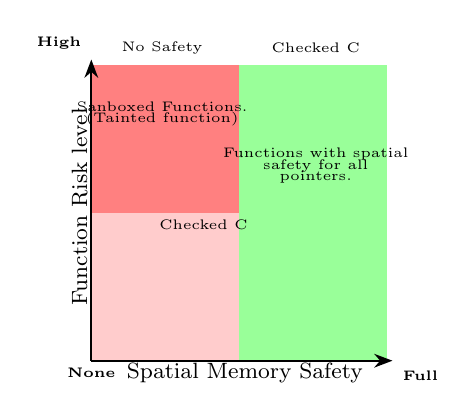
\begin{tikzpicture}[scale=0.75]
%\node[text width=3cm] at (1.5,-0.5) 
%    {some text spanning three};
%\draw[step=5cm,gray,very thin] (0,0) grid (5,5);


% This is all not protected region.
%Top left: High risk and low safety
\fill[red!50!white] (0,2.5) rectangle (2.5,5);
% bottom left: low risk and low safety
\fill[red!20!white] (0,0) rectangle (2.5,2.5);

% This is all protected.
% Top right: High risk and high safety
\fill[green!40!white] (2.5,2.5) rectangle (5,5);
% bottom right: low risk and high safety
\fill[green!40!white] (2.5,0) rectangle (5,2.5);


% High risk, high safety
\Text[x=3.8cm,y=5.3cm,fontsize=\footnotesize]{\tiny Checked C}
\Text[x=3.8cm,y=3.5cm,fontsize=\footnotesize]{\tiny Functions with spatial}
\Text[x=3.8cm,y=3.3cm,fontsize=\footnotesize]{\tiny safety for all}
\Text[x=3.8cm,y=3.1cm,fontsize=\footnotesize]{\tiny pointers.}

\Text[x=1.2cm,y=5.3cm,fontsize=\footnotesize]{\tiny No Safety}
\Text[x=1.2cm,y=4.3cm,fontsize=\footnotesize]{\tiny Sanboxed Functions.}
\Text[x=1.2cm,y=4.1cm,fontsize=\footnotesize]{\tiny (Tainted function)}

\Text[x=1.9cm,y=2.3cm,fontsize=\footnotesize]{\tiny Checked C}


%\Text[x=3.8cm,y=2.1cm,fontsize=\footnotesize]{\tiny Retrofitting}
%\Text[x=3.8cm,y=1.8cm,fontsize=\footnotesize]{\tiny Techniques.}
%\Text[x=3.8cm,y=1.5cm,fontsize=\footnotesize]{\tiny (ASAN, CCured,}
%\Text[x=3.8cm,y=1.3cm,fontsize=\footnotesize]{\tiny etc)}

%\Text[x=0.9cm,y=0.6cm,fontsize=\footnotesize]{\bf \faFlagCheckered}

%\Text[x=2.0cm,y=1.4cm,fontsize=\footnotesize]{\bf \footnotesize iC3C}

%\draw [{Implies}-,double,line width=1pt] (1.0,0.8) -- (1.9,2.1);


\draw[-Stealth,thick] (0,0) -- (5.1,0) node[anchor=north west] {\bf \tiny Full};
\Text[x=0cm,y=-0.2cm,fontsize=\footnotesize]{\bf \tiny None}
\Text[x=2.6cm,y=-0.2cm,fontsize=\footnotesize]{Spatial Memory Safety}
\Text[x=-0.2,y=2.6,rotation=90,fontsize=\footnotesize]{Function Risk level}
\draw[-Stealth,thick] (0,0) -- (0,5.1) node[anchor=south east] {\bf \tiny High};
\end{tikzpicture}
\caption{Existing approaches and the desired approach (\faFlagCheckered) along with our proposal (iC3C) to achieve it.}
\label{fig:tainedsplit}
\end{center}
\end{figure}





%\begin{listing*}[t!]
%\inputminted[linenos, mathescape, escapeinside=||, fontsize=\tiny{}]{c}{examples/originalprogram.c}
%\caption{Simple server example.}
%\label{lst:comb}
%\end{listing*}



\input{sections/content}

\section{Related Work}
% Safe C dialects and Checked C
Existing instrumentation based memory safety retrofitting techniques~\cite{duck2016heap,serebryany2012addresssanitizer,
  nagarakatte2009softbound,kendall1983bcc,steffen1992adding} add significant overhead~\cite{duck2016heap,serebryany2012addresssanitizer,
  nagarakatte2009softbound,kendall1983bcc,steffen1992adding}.
CCured~\cite{necula2005ccured}  and its successor Deputy~\cite{condit2007dependent}
aims to reduce overhead by adding checks only where
needed.
Nonetheless, unconverted pointers in CCured require extra metadata for pointers causing backward compatibility issues.
On the other hand, Checked C has no overhead and also is backward compatible.
% RLBox and related works
\systemname provides a Software Fault Isolation (SFI)~\cite{tan2017principles} mechanism for arbitrary functions in a program.
It uses a sandbox technique to enforce isolation.
There has been a considerable amount of work done in the area, especially for browsers~\cite{minsfi,barth-et-al:chromium:08, site-isolation-usenix}, which constantly runs code from potentially untrusted entities.
However, all these techniques use process/program-level isolation~\cite{site-isolation-usenix} and are not suited for seamlessly isolating parts of the same program.

Similar to RLBox, there are other works that provide sandboxing APIs.
These sandboxing mechanisms have different performance trade-offs \cite{wahbe-et-al:sfi:sosp93, nacl-amd64, minsfi, wasm,erim, tan-sfi-survey, shu-isolation-survey}. 
However, unlike RLBox, which enforces constraints 
through~\code{tainted} types, the other works have no such restrictions and expect the developer to take care of attacks from sandboxed regions explicitly.
% what does CheckCBox does on top of RLBox? What it provides? We should add that.
\systemname borrows the~\code{tainted} types from RLBox and merges them with Checked C types.
This enables us to have a more efficient sandboxing mechanism..what else?
\aravind{Fill this part.}

Our workflow of interactive type annotations has been explored before and is shown as an effective technique to assist developers in code conversion~\cite{machiry2022c} and vulnerability finding tasks~\cite{naik2021sporq}.

%%
%% The next two lines define the bibliography style to be used, and
%% the bibliography file.
\bibliographystyle{ACM-Reference-Format}
\bibliography{references, aravind, rlbox}



\end{document}
%%
%% End of file `sample-sigconf.tex'.
